% -*- Mode:TeX -*-


\documentclass[11pt,twoside,singlespace]{report}
%\pagestyle{plain}
%\pagestyle{headings}
%\lhead{\chaptermark}
\usepackage{bm}
\usepackage{commath}
\usepackage{amssymb,amsmath} % better maths commands
\usepackage{graphicx}
\usepackage{verbatim}  % allows 'comment' environment, which is useful for commenting out multi-line sections
%\usepackage{txfontsb}
\usepackage{mymanual}
\graphicspath{{graphics/}}
\usepackage[usenames]{color}
%\maxtocdepth{section}
\usepackage[sort&compress,numbers]{natbib} % better citations
\usepackage{fancyhdr}
%\usepackage[nottoc,notlot,notlof]{tocbibind}
\usepackage{url}
\usepackage{hyperref}
\hypersetup{colorlinks=true,linkcolor=blue}

\newcommand{\vv}{\upsilon}
\newcommand{\vect}[1]{{\mathbf #1}}
\newcommand{\regcoil}{{\ttfamily regcoil}}
\newcommand{\regcoilPlot}{{\ttfamily regcoilPlot}}
\newcommand{\netCDF}{{\ttfamily netCDF}}
\newcommand{\fortran}{{\ttfamily fortran}}
\newcommand{\matlab}{{\ttfamily matlab}}
\newcommand{\python}{{\ttfamily python}}
\newcommand{\nescoil}{{\ttfamily nescoil}}
\newcommand{\bnorm}{{\ttfamily bnorm}}
\newcommand{\nfp}{{\ttfamily nfp}}
\newcommand{\parlink}[1]{{\ttfamily \hyperlink{#1}{#1}}}
\newcommand{\vmec}{{\ttfamily vmec}}
\newcommand{\todo}[1]{\textcolor{red}{To do: #1}}

\graphicspath{{figures/}}

% uncomment the following line to remove all graphics (for faster compiling)
%\renewcommand{\includegraphics}[2][x]{}

\newcommand{\boldkappa}{{\mathbf \kappa}}

\setlength{\oddsidemargin}{0.25in}	% 1.25in left margin
\setlength{\evensidemargin}{0.25in}	% 1.25in left margin (even pages)
\setlength{\topmargin}{0.0in}		% 1in top margin
\setlength{\textwidth}{6.0in}		% 6.0in text - 1.25in rt margin
\setlength{\textheight}{8.6in}		% Body ht for 1in margins

\setcounter{tocdepth}{1}
\begin{document}


\begin{center}

\vspace*{1in}

{\Huge REGCOIL User Manual}

\vspace{2in}

\centerline{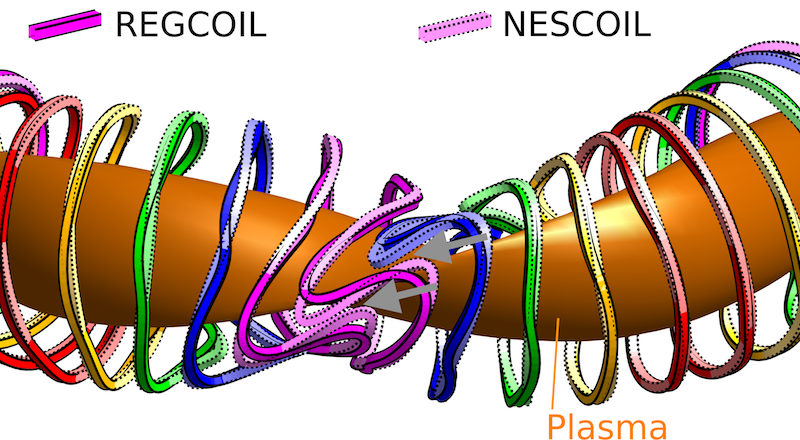
\includegraphics[width=6.5in]{m20170111_01_compareNescoilToRegcoilCoils.png}}

%{\Large Version 3}

\vspace{1.0in}

Revised May 15, 2019

\end{center}




%\pagestyle{plain}
\fancyhf{}
\cfoot{\thepage}
\tableofcontents

\clearpage


\pagestyle{fancy}
\fancyhf{}
\lhead[\thepage]{\leftmark}
\rhead[\leftmark]{\thepage}
%\lhead{\chaptermark}
\renewcommand{\chaptermark}[1]{\markboth{\sc{\chaptername\ \thechapter.\ #1}}{}}
\setlength{\headsep}{6pt}

\setlength{\parskip}{0pt plus 0pt minus 0pt}

% Main chapters go here:
\chapter{Overview}

This program is an implementation of the \regcoil~algorithm described in \cite{regcoilPaper},
and was used for the calculations in \cite{regcoilPaper}.
This paper is available in the Git repository for this program.
In addition, this program can read output files from the \nescoil~code \cite{nescoil},
processing the results to compute quantities like the current density
and residual magnetic field normal to the target plasma surface.

%In the various variable names in the code and output file, `r' refers
%to the position vector, not to a radius.  In various arrays with a
%dimension of length 3, this dimension always corresponds to Cartesian
%coordinates $(x,y,z)$.

%The `normal' quantities in the code and output file refer to the
%surface normal vector N = (dr/dv) cross (dr/du) as in the NESCOIL
%paper. Note that this vector does not have unit magnitude.



\section{Required libraries}

\begin{itemize}

\item {\ttfamily NetCDF} (for writing the output file)
\item {\ttfamily BLAS} (for matrix multiplication)
\item {\ttfamily LAPACK} (for solving linear systems and for singular value decomposiiton)

\end{itemize}

Most of these libraries will be available on any high-performace computing system. {\ttfamily BLAS} and {\ttfamily LAPACK}
are available on Apple Mac computers (as part of the Accelerate framework) if you install Xcode through the App store.

If {\ttfamily OpenMP} is available, calculations with the code are parallelized.
The plotting and testing functions use \python,
{\ttfamily numpy}, and {\ttfamily scipy}.
The plotting routines \regcoilPlot~and {\ttfamily compareRegcoil} use {\ttfamily matplotlib}.

\section{Parallelization}

The code does not use {\ttfamily MPI}, and so it runs on a single computing node.  However, it is possible to use multiple threads
on the node to accelerate computations.  The multi-threaded parallelization is done in part using {\ttfamily OpenMP}
and in part using a multi-threaded {\ttfamily BLAS} routine. Typically the number of threads is set by
setting the environment variable {\ttfamily OMP\_NUM\_THREADS}.

%The slowest steps in \regcoil~are typically the assembly of the
%matrices described in appendix B of \cite{regcoilPaper}.  For each of these two matrices, there are two slow steps.
%The first is computation of the magnetic dipole formula between each pair of points
%on the two toroidal surfaces.  The loop for this computation is parallelized using {\ttfamily OpenMP}.
%The other slow step is the integration of this result against Fourier modes,
%which is done using matrix multiplication with the {\ttfamily BLAS} subroutine {\ttfamily DGEMM}.
%To parallelize this step you can link \regcoil~with a multi-threaded  {\ttfamily BLAS} library,
%such as the Intel Math Kernel Library (MKL).

\section{\ttfamily make test}

To test that your \regcoil~executable is working, you can run {\ttfamily make test}.  Doing so will run
\regcoil~for some or all of the examples in the {\ttfamily examples/} directories.
After each example completes, several of the output quantities
will be checked, using the
{\ttfamily tests.py} script in the example's directory.
The {\ttfamily make test} feature is very useful when making changes to the code, since it allows you to check
that your code modifications have not broken anything and that previous results
can be recovered.

If you run {\ttfamily make retest},
no new runs of \regcoil~will be performed, but the {\ttfamily tests.py} script
will be run on any existing output files in the \path{/examples/} directories.

\section{Units}

As in \vmec, all of \regcoil's input and output parameters use SI units: meters, Teslas, Amperes, and combinations thereof.

\section{Plasma current}

If there is current inside the plasma, then this current will contribute to the magnetic field normal
to the target plasma surface, which the coils must cancel. The contribution of plasma current to the normal field
is not computed directly by \regcoil, but it can be computed using the \bnorm~code which is 
often distributed with \vmec.  You can then set \parlink{load\_bnorm}={\ttfamily .true.} and specify \parlink{bnorm\_filename}
in the \regcoil~input namelist to load the \bnorm~results into \regcoil.

\section{Matlab version}

Both \fortran~and \matlab~versions of \regcoil~are included in the repository.  The \matlab~version is
contained in the file {\ttfamily regcoil.m}. For normal
use you will want to use the \fortran~version, since it is much faster.  The \matlab~version was originally
written as a check of the \fortran~version, to verify that two independent implementations of the algorithm
in different languages give identical results.  The \matlab~version reads in an output file from the \fortran~version
and verifies that each significant variable is identical.  A few of the features in the \fortran~version
are not available in the \matlab~version.

\section{Plotting results}

The python program \regcoilPlot~will display many of the output quantities from a single \regcoil~calculation.
Results from multiple \regcoil~calculations can be compared using the python program {\ttfamily compareRegcoil}.

You can also make a 3D figure of the shapes of discrete coils using the \matlab~program {\ttfamily m20160811\_01\_plotCoilsFromRegcoil.m}.
Two different sets of coils can be plotted together using the \matlab~program {\ttfamily m20160811\_02\_compare2CoilsetsFromRegcoil.m}.
The latter program was used to generate the figure on the cover of this manual.

\section{Cutting coils}

Once a suitable current potential has been computed with \regcoil, you can `cut' discrete coils
using the python script {\ttfamily cutCoilsFromRegcoil}. You can run this script with no arguments
to see a list of the input parameters. This script will generate a coils file suitable for input to the
{\ttfamily makegrid} code (distributed with \vmec), which in turn generates an mgrid file used as input for free-boundary \vmec.

\section{Questions, Bugs, and Feedback}

We welcome any contributions to the code or documentation.
For write permission to the repository, or to report any bugs, provide feedback, or ask questions, contact Matt Landreman at
\href{mailto:matt.landreman@gmail.com}{\nolinkurl{matt.landreman@gmail.com} }







\chapter{Input Parameters}
\label{ch:input}

\newcommand{\param}[5]{{\setlength{\parindent}{0cm} {\ttfamily \bfseries \hypertarget{#1}{#1}}\\{\it Type}: #2\\{\it Default}: #3\\{\it When it matters}: #4\\{\it Meaning}: #5}}
\newcommand{\myhrule}{{\setlength{\parindent}{0cm} \hrulefill }}

\newcommand{\true}{{\ttfamily .true.}}
\newcommand{\false}{{\ttfamily .false.}}

In this section we describe all the parameters which can be included in the input namelist. 

\section{General parameters}

\param{general\_option}
{integer}
{1}
{Always}
{Determines the overall flow of program execution.\\

{\ttfamily general\_option} = 1: Compute the current potential for a range of $\lambda$.\\

{\ttfamily general\_option} = 2: Do not compute the current potential, but rather load the current potential computed
by \nescoil~in the file \parlink{nescout\_filename}, compute the $\chi^2_B$ and $\chi^2_K$ for it,
and save results. For this setting, \parlink{Nlambda} will be over-written with the number of
current potential solutions found in the nescout file.\\

{\ttfamily general\_option} = 3: Emulate \nescoil's truncated singular value decomposition (TSVD) solver.
The least-squares problem solved will be minimization of only $\chi^2_B$ (i.e. $\lambda=0$.)
Output quantities will be saved in the same arrays as if $\lambda$ were scanned.
For this setting, \parlink{Nlambda} will be over-written with the number of
singular values.\\

{\ttfamily general\_option} = 4: Search for a value of the regularization weight such that
a certain target is met. The target is chosen using \parlink{target\_option}.
Use this value of {\ttfamily general\_option} for running \regcoil~inside
a fixed-boundary plasma shape optimization, in which case {\ttfamily chi2\_B\_target}
is the objective function you should minimize in the optimization.\\

{\ttfamily general\_option} = 5: Same as 4, except that before the $\lambda$ search is carried out,
the system is solved
for $\lambda=0$ and $\lambda=\infty$ to check whether the current density target is attainable.
Thus, this option takes a little more time than {\ttfamily general\_option}=4 but is more robust.
}

\myhrule

\param{nescout\_filename}
{string}
{`'}
{Only when \parlink{general\_option}=2.}
{Name of a \nescoil~output file which can be read in for processing.
}

\myhrule

\param{symmetry\_option}
{integer}
{1}
{Always}
{Determines whether stellarator symmetry is imposed.\\

{\ttfamily symmetry\_option} = 1: Force the single-valued part of the current potential
to be odd in $\theta$ and $\zeta$. This option corresponds to stellarator symmetry.\\

{\ttfamily symmetry\_option} = 2: Force the single-valued part of the current potential
to be even in $\theta$ and $\zeta$. I'm not sure why you would ever use this option,
but it is available for completeness.\\

{\ttfamily symmetry\_option} = 3: No symmetry in the current potential is imposed.
}

\myhrule

\param{save\_level}
{integer}
{3}
{Always}
{Option related determining how many variables are saved in the \netCDF~output file.  The larger the value, the smaller the output file.\\

{\ttfamily save\_level} = 0: Save everything.\\

{\ttfamily save\_level} = 1: Do not save the inductance matrix.\\

{\ttfamily save\_level} = 2: Also do not save the matrix $g$.\\

{\ttfamily save\_level} = 3: Also do not save the normal vector or derivatives of the position vector.
}

\myhrule

\param{load\_bnorm}
{logical}
{\false}
{When \parlink{general\_option}=1 or 3.}
{Whether or not an output file from the \bnorm~code is to be loaded.
Set this option to \true~if there is significant current in the plasma,
meaning the coils will need to cancel the associated magnetic field component normal
to the target plasma surface.
}

\myhrule

\param{bnorm\_filename}
{string}
{`'}
{When \parlink{general\_option}=1 or 3 and \parlink{load\_bnorm}=\true.}
{Output file from the \bnorm~code which contains the magnetic field normal to the target
plasma surface associated with current inside the plasma.}

\myhrule

\param{net\_poloidal\_current\_Amperes}
{real}
{1.0}
{If \parlink{geometry\_option\_plasma}=0,1,or 5, i.e. if the plasma surface is not a vmec equilibrium.}
{The number of Amperes of current the links the coil winding surface poloidally,
denoted $G$ in \cite{regcoilPaper}. If the plasma surface is obtained from a vmec equilibrium,
then {\ttfamily net\_poloidal\_current\_Amperes} will be determined instead
from the {\ttfamily bvco} value in the vmec wout file.
}

\myhrule

\param{net\_toroidal\_current\_Amperes}
{real}
{0.0}
{Always}
{The number of Amperes of current the links the coil winding surface toroidally,
denoted $I$ in \cite{regcoilPaper}. Unlike the net poloidal current, this number
is never read from a wout file.
}



\section{Resolution parameters}

For any new set of surface geometries you consider, you should vary the resolution parameters in this section to make sure
they are large enough.  These parameters should be large enough that the code results you care about are unchanged under further
resolution increases.

\myhrule

\param{ntheta\_plasma}
{integer}
{64}
{Always}
{Number of grid points in poloidal angle used to evaluate surface integrals on the plasma surface.
Often 64 or 128 is a good value.
It is resonable and common but not mandatory to use the same value for {\ttfamily ntheta\_plasma} and \parlink{ntheta\_coil}.}

\myhrule

\param{ntheta\_coil}
{integer}
{64}
{Always}
{Number of grid points in poloidal angle used to evaluate surface integrals on the coil winding surface.
Often 64 or 128 is a good value.
It is resonable and common but not mandatory to use the same value for \parlink{ntheta\_plasma} and {\ttfamily ntheta\_coil}.}

\myhrule


\param{nzeta\_plasma}
{integer}
{64}
{Always}
{Number of grid points in toroidal angle used to evaluate surface integrals on the plasma surface.
Often 64 or 128 is a good value.
It is resonable and common but not mandatory to use the same value for {\ttfamily nzeta\_plasma} and \parlink{nzeta\_coil}.}

\myhrule

\param{nzeta\_coil}
{integer}
{64}
{Always}
{Number of grid points in toroidal angle used to evaluate surface integrals on the coil winding surface.
Often 64 or 128 is a good value.
It is resonable and common but not mandatory to use the same value for \parlink{nzeta\_plasma} and {\ttfamily nzeta\_coil}.}

\myhrule

\param{mpol\_coil}
{integer}
{12}
{Always}
{Maximum poloidal mode number to include for the single-valued part of the current potential on the coil winding surface.
}

\myhrule

\param{ntor\_coil}
{integer}
{12}
{Always}
{
Maximum toroidal mode number to include for the single-valued part of the current potential on the coil winding surface.
}

\myhrule

\param{mpol\_transform\_refinement}
{real}
{5.0}
{Only when \parlink{geometry\_option\_plasma} is 4.}
{The number of poloidal mode numbers in the \vmec~file will be multiplied by this value
when transforming from the original poloidal angle to the straight-field-line angle.
Since the original \vmec~angle is chosen to minimize the number of Fourier modes required,
more modes are required in any other coordinate.
This parameter affects the time required to compute constant-offset surfaces,
but does not affect the time for other calculations.
}

\myhrule

\param{ntor\_transform\_refinement}
{real}
{1.0}
{Only when \parlink{geometry\_option\_plasma} is 4.}
{The number of toroidal mode numbers in the \vmec~file will be multiplied by this value
when transforming from the original poloidal angle to the straight-field-line angle.
Since the original \vmec~angle is chosen to minimize the number of Fourier modes required,
more modes are required in any other coordinate.
This parameter affects the time required to compute constant-offset surfaces,
but does not affect the time for other calculations.
}

\section{Geometry parameters for the plasma surface}

\param{geometry\_option\_plasma}
{integer}
{0}
{Always}
{This option controls how you specify the shape of the target plasma surface.\\

{\ttfamily geometry\_option\_plasma} = 0: The plasma surface will be a plain circular torus. The major radius will be \parlink{R0\_plasma}.
     The minor radius will be \parlink{a\_plasma}. This option exists just for testing purposes.\\

{\ttfamily geometry\_option\_plasma} = 1: Identical to option 0.\\

{\ttfamily geometry\_option\_plasma} = 2: The plasma surface will be the last surface in the full radial grid of the \vmec~file specified by \parlink{wout\_ilename}.
The poloidal angle used will be the normal \vmec~angle which is not a straight-field-line coordinate.
This is typically the best option to use for working with \vmec~equilibria.\\

{\ttfamily geometry\_option\_plasma} = 3: The plasma surface will be the last surface in the half radial grid of the \vmec~file specified by \parlink{wout\_filename}.
The poloidal angle used will be the normal \vmec~angle which is not a straight-field-line coordinate.
This option exists so that the same flux surface can be used when comparing with {\ttfamily geometry\_option\_plasma} = 4.\\

{\ttfamily geometry\_option\_plasma} = 4: The plasma surface will be the last surface in the half radial grid of the \vmec~file specified by \parlink{wout\_filename}.
The poloidal angle used will be the straight-field-line coordinate, obtained by shifting the normal \vmec~poloidal angle by \vmec's $\lambda$ quantity.
This option exists in order to examine changes when using a different poloidal coordinate compared to {\ttfamily geometry\_option\_plasma} = 3.\\

{\ttfamily geometry\_option\_plasma} = 5: The plasma surface will be the flux surface with normalized poloidal flux
\parlink{efit\_psiN} taken from the {\ttfamily efit} file specified by \parlink{efit\_filename}. \\

{\ttfamily geometry\_option\_plasma} = 6: The plasma surface will be loaded from an ASCII file, specified by \parlink{shape\_filename\_plasma}. The first line of this file is ignored. The second line is an integer giving the number of Fourier modes
to read. The remaining lines contain $m$, $n$, $rmnc$, $zmns$, $rmns$, $zmnc$.
}

\myhrule

\param{shape\_filename\_plasma}
{string}
{`'}
{Only when \parlink{geometry\_option\_plasma} is 6.}
{ASCII file from which to read in the plasma shape.}

\myhrule

\param{R0\_plasma}
{real}
{10.0}
{Only when \parlink{geometry\_option\_plasma} is 0 or 1.}
{Major radius of the plasma surface, when this surface is a plain circular torus.}

\myhrule

\param{a\_plasma}
{real}
{0.5}
{Only when \parlink{geometry\_option\_plasma} is 0 or 1.}
{Minor radius of the plasma surface, when this surface is a plain circular torus.}

\myhrule

\param{nfp\_imposed}
{integer}
{1}
{Only when \parlink{geometry\_option\_plasma} is 0 or 1.}
{When the plasma surface is a plain circular torus, only toroidal mode numbers that are a multiple of this parameter will be considered.
This parameter thus plays a role like \vmec's {\ttfamily nfp} (number of field periods),
and is used when {\ttfamily nfp} is not already loaded from a \vmec~file.}

\myhrule

\param{wout\_filename}
{string}
{`'}
{Only when \parlink{geometry\_option\_plasma} is 2, 3, or 4.}
{Name of the \vmec~{\ttfamily wout} output file which will be used for the plasma surface.
You can use either a \netCDF~or {\ttfamily ASCII} format file.}

\myhrule

\param{efit\_filename}
{string}
{`'}
{Only when \parlink{geometry\_option\_plasma} is 5.}
{Name of the {\ttfamily efit} output file which will be used for the plasma surface.}

\myhrule

\param{efit\_psiN}
{real}
{0.98}
{Only when \parlink{geometry\_option\_plasma} is 5.}
{Value of normalized poloidal flux at which to select a flux surface from the {\ttfamily efit} input file.
A value of 1 corresponds to the last closed flux surface, and 0 corresponds to the magnetic axis.}

\myhrule

\param{efit\_num\_modes}
{integer}
{10}
{Only when \parlink{geometry\_option\_plasma} is 5.}
{Controls the number of Fourier modes used to represent $R(\theta)$ and $Z(\theta)$ for the shape of
the plasma surface. Each of these functions will be expanded in a sum of functions $\sin(m\theta)$ and $\cos(m\theta)$,
where $m$ ranges from 0 to {\ttfamily efit\_num\_modes}$-1$.}

\section{Geometry parameters for the coil winding surface}

\param{geometry\_option\_coil}
{integer}
{0}
{Always}
{This option controls which type of geometry is used for the coil surface.\\

{\ttfamily geometry\_option\_coil} = 0: The coil surface will be a plain circular torus. The major radius will be the 
same as the plasma surface: either \parlink{R0\_plasma} if \parlink{geometry\_option\_plasma} is 0 or 1, or {\ttfamily Rmajor\_p} from the \vmec~{\ttfamily wout} file
if  \parlink{geometry\_option\_plasma} is 2.
     The minor radius will be \parlink{a\_coil}.\\

{\ttfamily geometry\_option\_coil} = 1: Identical to option 0, except the major radius of the coil surface will be set by \parlink{R0\_coil}.\\

{\ttfamily geometry\_option\_coil} = 2: The coil surface will computing by expanding the plasma surface uniformly by a distance \parlink{separation}.\\

{\ttfamily geometry\_option\_coil} = 3: The coil surface will be the `coil' surface in the \nescoil~`nescin' input file specified by \parlink{nescin\_filename}.
}

\myhrule

\param{R0\_coil}
{real}
{10.0}
{Only when \parlink{geometry\_option\_coil} is 1.}
{Major radius of the coil surface, when this surface is a plain circular torus.}

\myhrule

\param{a\_coil}
{real}
{1.0}
{Only when \parlink{geometry\_option\_coil} is 0 or 1.}
{Minor radius of the coil surface, when this surface is a plain circular torus.}


\myhrule

\param{separation}
{real}
{0.2}
{Only when \parlink{geometry\_option\_coil} is 2.}
{Amount by which the coil surface is offset from the plasma surface.}

\myhrule

\param{nescin\_filename}
{string}
{`'}
{Only when \parlink{geometry\_option\_coil} is 3.}
{Name of a \nescoil~{\ttfamily nescin} input file. The coil surface from
this file will be used as the coil surface for \regcoil.}

\myhrule

\param{save\_nescin\_option}
{integer}
{0}
{When \parlink{geometry\_option\_coil = 2}.}
{Determines whether or not to save the offset surface coefficients in nescin format. Stellarator symmetry is assumed. \\
{\ttfamily save\_nescin\_option} = 0: No nescin file is saved. \\
{\ttfamily save\_nescin\_option} = 1: Nescin file is saved with name \texttt{nescin.offset}. }

\myhrule

\param{save\_nescin\_mpol}
{integer}
{12}
{When \parlink{save\_nescin\_option =1}. }
{Number of poloidal Fourier modes for the nescin file.}

\myhrule

\param{save\_nescin\_ntor}
{integer}
{12}
{When \parlink{save\_nescin\_option = 1}.}
{Number of toroidal Fourier modes for the nescin file.}


\section{Parameters related to the regularization weight}

\param{Nlambda}
{integer}
{4}
{Only when \parlink{general\_option}=1, 4, or 5.}
{When \parlink{general\_option}=1, {\ttfamily Nlambda} is the number of values of $\lambda$ for which the problem is solved.
When \parlink{general\_option}=4 or 5, {\ttfamily Nlambda} is the upper limit on the number of values of $\lambda$ for which the problem is solved.}

\myhrule

\param{lambda\_max}
{real}
{1.0e-13}
{Only when \parlink{general\_option}=1.}
{Maximum value of $\lambda$ for which the problem is solved.}

\myhrule

\param{lambda\_min}
{real}
{1.0e-19}
{Only when \parlink{general\_option}=1.}
{Minimum nonzero value of $\lambda$ for which the problem is solved.
Note that the problem is always solved for $\lambda=0$ in addition to
the nonzero values.}

\myhrule

\param{target\_option}
{integer}
{1}
{Only when \parlink{general\_option}=4 or 5.}
{Controls which target is used to find determine $\lambda$:\\

{\ttfamily target\_option} = 2: Search for the $\lambda$ value such that the maximum
current density over the winding surface equals \parlink{current\_density\_target}.\\

{\ttfamily target\_option} = 1: Search for the $\lambda$ value such that the root-mean-square current density
$\left( \int d^2a\; K^2 \right)^{1/2}$ equals \parlink{current\_density\_target}.
}

\myhrule

\param{current\_density\_target}
{real}
{8.0e6}
{Only when \parlink{general\_option}=4 or 5.}
{The value of root-mean-square or maximum surface current density used to determine $\lambda$.
See \parlink{target\_option}.
As with all other input and output quantities, this surface current density is specified in SI units,
so the units are Amperes/meter.
}

\myhrule

\param{lambda\_search\_tolerance}
{real}
{1.0e-5}
{Only when \parlink{general\_option}=4 or 5.}
{Relative tolerance for the lambda root-finding.}

\myhrule

\section{Parameters Related to Sensitivity \& Adjoint Solve}

\myhrule

\param{sensitivity\_option}
{integer}
{1}
{If gradients of with respect to coil geometry parameters are desired.}
{\\ Currently, the derivatives with respect to geometry are performed at constant $\lambda$. \texttt{sensitivity\_option = 3,4,5} should give the same results, though \texttt{sensitivity\_option=5} tends to be the most efficient. \\ \\
\texttt{sensitivity\_option = 1}: No sensitivity information is computed. \\ \\
\texttt{sensitivity\_option = 2}: Sensitivity of $\chi^2$ is computed. The same range of $\lambda$ is used as that designated by \parlink{Nlambda}, \parlink{lambda\_max}, and \parlink{lambda\_min}. \\ \\
\texttt{sensitivity\_option = 3}: Sensitivity of $\chi^2_K$ and $\chi^2_B$ are computed in addition to that of $\chi^2$. This requires two adjoint solves. \\ \\
\texttt{sensitivity\_option = 4}: Sensitivity of $\chi^2_K$ and $\chi^2_B$ are computed in addition to that of $\chi^2$. An adjoint solve is used to compute the sensitivity of $\chi^2_K$, and the sensitivity of $\chi^2_B$ is computed by subtracting $\lambda \partder{\chi^2_K}{\Omega}$ from $\partder{\chi^2}{\Omega}$. This requires one adjoint solve. \\ \\
\texttt{sensitivity\_option = 5}: Sensitivity of $\chi^2_K$ and $\chi^2_B$ are computed in addition to that of $\chi^2$. An adjoint solve is used to compute the sensitivity of $\chi^2_B$, and the sensitivity of $\chi^2_K$ is computed by subtracting $\partder{\chi^2_B}{\Omega}$ from $\partder{\chi^2}{\Omega}$ and dividing by $\lambda$. 
}
%\texttt{sensitivity_option == 2}: Sensitivity of $\chi^2$ is computed. The same $\lambda$ is used as that designated by \parlink{Nlambda}, \parlink{lambda\_max}, and \parlink{lambda\_min}. 
%}

\myhrule

\param{normal\_displacement\_option}
{integer}
{0}
{When \parlink{sensitivity\_option} $>1$.}
{This provides an option to compute the normal component of the sensitivity of $\chi^2$, $\chi^2_K$ and $\chi^2_B$ as a function of position on the coil-winding surface. \textcolor{red}{Neither \texttt{normal\_displacement\_option = 1} or 2 give reliable results at this point.} \\ \\ 
\texttt{normal\_displacement\_option = 0}: Normal displacement diagnostic is not computed. \\ \\
\texttt{normal\_displacement\_option = 1}: Normal displacement diagnostic is computed use Fourier transform approach \\ \\
\texttt{normal\_displacement\_option = 2}: Normal displacement diagnostic is computed using SVD approach.}

\myhrule

\param{nmax\_sensitivity}
{integer}
{0}
{When \parlink{sensitivity\_option} $> 1$.}
{Sensitivity of $\chi^2$, $\chi^2_B$, and $\chi^2_K$ will be computed with respect to $r_{mn}^c$ and $z_{mn}^s$ for $\abs{n} \leq $ \texttt{nmax\_sensitivity}.}

\myhrule

\param{mmax\_sensitivity}
{integer}
{0}
{When \parlink{sensitivity\_option} $> 1$.}
{Sensitivity of $\chi^2$, $\chi^2_B$, and $\chi^2_K$ will be computed with respect to $r_{mn}^c$ and $z_{mn}^s$ for $m \leq $ \texttt{nmax\_sensitivity}.}

\myhrule

\param{sensitivity\_symmetry\_option}
{integer}
{1}
{When \parlink{sensitivity\_option} $> 1$.}
{Symmetry assumed when computed sensitivity to coil geometry parameters. This does not need to be the same as \parlink{symmetry\_option}. \\
{\ttfamily sensitivity\_symmetry\_option} = 1: Force the single-valued part of the current potential
to be odd in $\theta$ and $\zeta$. This option corresponds to stellarator symmetry.\\

{\ttfamily sensitivity\_symmetry\_option} = 2: Force the single-valued part of the current potential
to be even in $\theta$ and $\zeta$. I'm not sure why you would ever use this option,
but it is available for completeness.\\

{\ttfamily sensitivity\_symmetry\_option} = 3: No symmetry in the current potential is imposed.
}


%\include{runs}
%\include{resolution} 

\renewcommand{\chaptermark}[1]{\markboth{\sc{Appendix\ \thechapter.\ #1}}{}}
\appendix
\setcounter{tocdepth}{0}

% Appendices can go here:
%\include{systems}
 
\lhead[\thepage]{\sc Bibliography}
\rhead[\sc Bibliography]{\thepage}
\bibliography{regcoilManual}
\bibliographystyle{mymanual}
\end{document}

